\textbf{- Reference:} 
\href{https://e.math.cornell.edu/people/belk/numbertheory/CyclotomicPolynomials.pdf}{Fields and Cyclotomic Polynomials}~\cite{cyclotomic-polynomial}


\subsection{Definitions}
\label{subsec:roots-def}
\begin{tcolorbox}[title={\textbf{\tboxdef{\ref*{subsec:roots-def}} Definitions for Roots of Unity}}]
\begin{itemize}
\item \textbf{$\bm{n}$-th root of Unity:} A complex number $\zeta$ that satisfies the equation $\zeta^n = 1$
\item \textbf{Primitive $\bm{n}$-th Root of Unity:} Any $n$-th root of unity $\zeta$ such that $\textsf{ord}_\mathbb{C}(\zeta) = n$. We denote $P(n)$ as a set of primitive $n$-th root of unity. 
\end{itemize}

$ $

A primitive $n$-th root of unity is considered a \textit{generator} of all $n$ $n$-th roots of unity.
\end{tcolorbox}

\subsection{Theorems}
\label{subsec:roots-theorem}


\begin{tcolorbox}[title={\textbf{\tboxtheorem{\ref*{subsec:roots-theorem}.1} Formula for $\bm{n}$-th Root of Unity}}]
Given $\zeta^n = 1$, there exist exactly $n$ different $n$-th roots of unity: 

$ $

$\zeta = e^{2k\pi i/n} = \cos\left(\dfrac{2k\pi}{n}\right) + i\cdot\sin\left(\dfrac{2k\pi}{n}\right)$, 

$ $

\noindent for $n$ different $k$ values, where $k = \{0, 1, \cdots, n-1\}$.
\end{tcolorbox}
\begin{myproof} 
    \begin{enumerate}
    \item Suppose $\zeta = e^{2k\pi i/n}$. Then, $\zeta^n = (e^{2k\pi i/n})^n = e^{2k\pi i}$, and since $\zeta^n = 1$, we need to find the $k$ values such that $e^{2k\pi i} = 1$
    \item Euler's formula states that $e^{i\cdot x} = \text{cos}(x) + i \cdot \text{sin}(x)$. Therefore, if $x = 2k\pi$, then $e^{2k\pi i} = \text{cos}(2k\pi) + i \cdot \text{sin}(2k\pi)$. This formula becomes 1 if $k = 0, 1, 2, ...$. Thus, $e^{2k\pi i} = 1$ for any integer $k \geq 0$. 
    \item If $\zeta = e^{2k\pi i/n} = \text{cos}(\frac{2k\pi}{n}) + i\cdot\text{sin}(\frac{2k\pi}{n})$, then the first $n$ roots for $k = 0, 1, ... \text{ } n-1$ are all distinct values, because they lie on the circle in the complex plane (where $x$-axis is a real value and $y$-axis is a complex value coefficient) at each angle $2k\pi/n$ for $k = \{0, 1, \cdots, n-1\}$.
    \item Note $\zeta^n = 1$ is an $n$-th polynomial, so it can have at most $n$ roots. Thus, we can consider the first $n$ roots $e^{2k\pi i/n}$ for $k = \{0, 1, \cdots, n-1\}$ as the $n$ distinct roots and ignore the rest of roots (i.e., $k \geq n$), considering them to be repetitions of the first $n$ roots on a circle in the complex plane (see \autoref{fig:complex-plane}). 
    \end{enumerate}
\end{myproof}

\begin{figure}[h!]
    \centering
  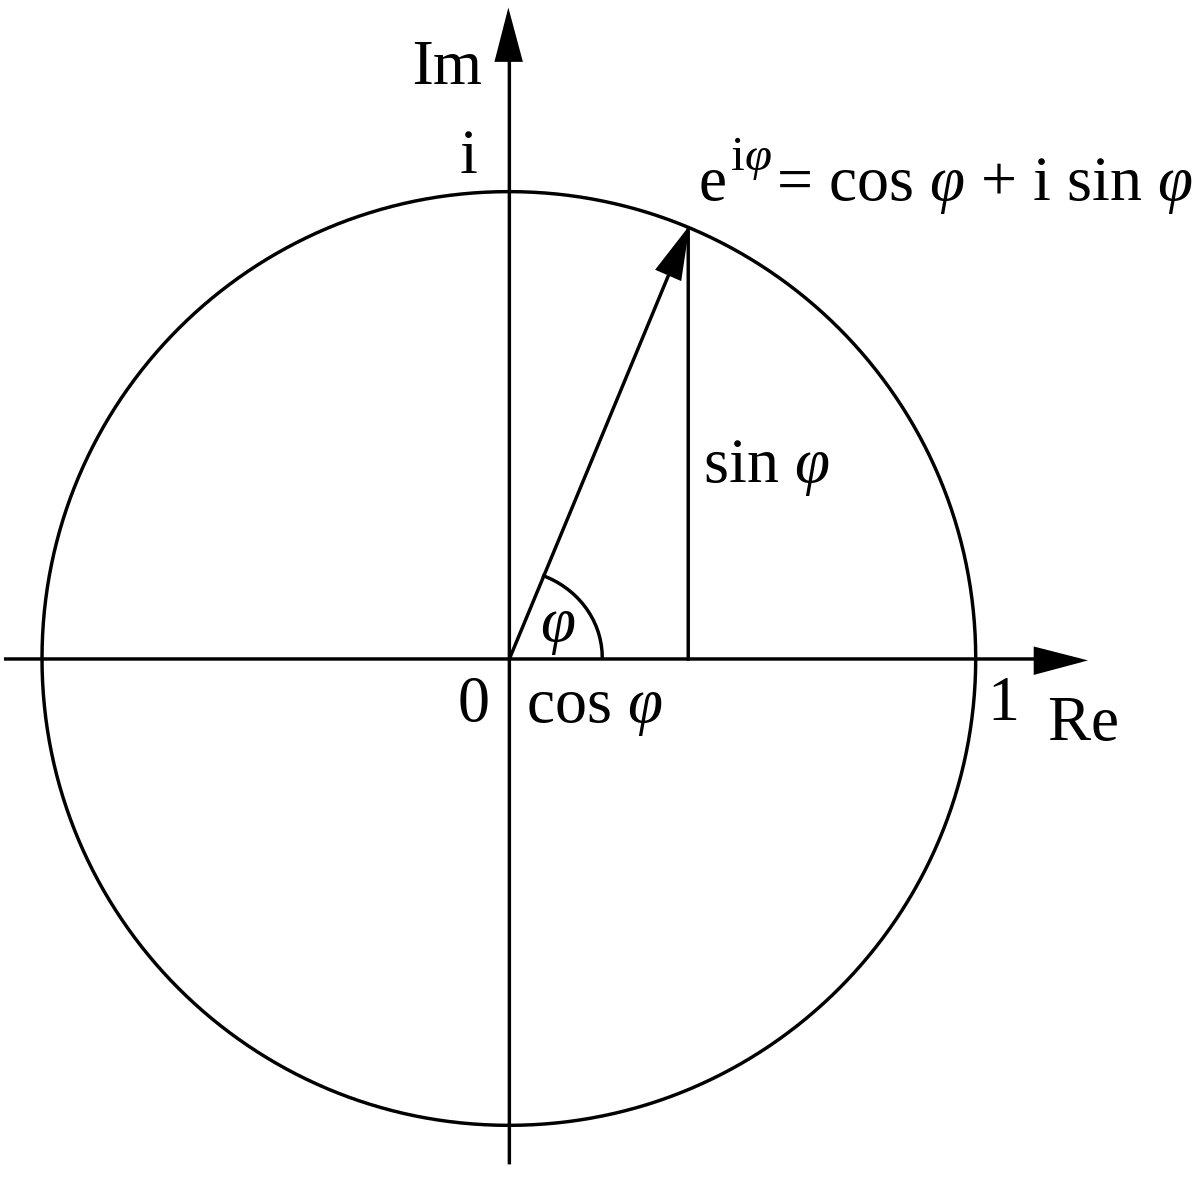
\includegraphics[width=0.4\linewidth]{figures/euler-formula.png}
  \caption{The figure illustrates a circle of Euler's formula in the complex plane \href{https://en.wikipedia.org/wiki/Euler's_formula}{(Source)}}
  \label{fig:complex-plane}
\end{figure}


\begin{tcolorbox}[title={\textbf{\tboxtheorem{\ref*{subsec:roots-theorem}.2} Order of the Root of Unity}}]
Given $\zeta \in \mathbb{C}$ (the complex number domain) and $\zeta^n = 1$ where $n \geq 1$, $\zeta$ is an $n$-th root of unity if and only if $\textsf{ord}_\mathbb{C}(\zeta) \text{ } | \text{ } n$.
\end{tcolorbox}
\begin{proof}
    We use 
    Theorem~\ref*{subsec:order-theorem}.1:
    \begin{enumerate}
    \item \textit{Forward Proof:} Since $\textsf{ord}_\mathbb{C}(\zeta)=k$ is the smallest integer such that $\zeta^k = 1$, for any $n$ that satisfies $\zeta^n = 1$, $n$ must be a multiple of $k$. This means that $k \gap{$|$} n$.
    \item \textit{Backward Proof:} If $k \gap{$|$} n$, then $n$ is a multiple of $k$, which means that $\zeta^n = 1$. 
    \end{enumerate}
    %$(Here, note that our \b\bmodulo computation wraps around a circle of Euler's formula on the complex plane instead of a finite integer field).
\end{proof}

\begin{tcolorbox}[title={\textbf{\tboxtheorem{\ref*{subsec:roots-theorem}.3} Set of All $\bm{n}$-th Roots of Unity}}]
The set of all $n$-th roots of unity is the union $\bigcup_{d|n} P(d)$ (i.e., the union of all primitive $d$-th roots of unity where $d \text{ } | \text{ } n$).
\end{tcolorbox}
\begin{myproof}
    \begin{enumerate}
    \item Let $\omega = e^{2\pi i/n}$.
    Given $\zeta^n = 1$, for each $n$-th root of unity $\zeta$ is, $\zeta = \omega^{k_i}$ for $k_i = \{0, 1, \cdots, n-1\}$. Note that according to Theorem~\ref*{subsec:order-theorem}.1, $(\omega^{k_i})^n = 1$ if and only if $\textsf{ord}_\mathbb{C}(\omega^{k_i}) \text{ } | \text{ } n$. 
    \item Let $\textsf{ord}_\mathbb{C}(\omega^{k_i}) = d_i$. Then, $(\omega^{k_i})^{d_i} = 1$. Combining these two facts, each $n$-th root of unity $\omega^{k_i}$ is also a primary $d_i$-th root of unity (i.e., a solution for $\zeta^{d_i} = 1$), that is, $\omega^{k_i} \in P(d_i)$. 
    \item Remember that for each $\textsf{ord}_\mathbb{F}(\omega^{k_i}) = d_i$, $d_i \text{ } | \text{ } n$. For every $d_i$ that divides $n$, all the (primary) $d_i$-th roots of unity are also the $n$-th root of unity. This is because the (primary) $d_i$-th root of unity that satisfies $\zeta^{d_i} = 1$ also satisfies $\zeta^{n} = 1$ (as $n$ is a multiple of $d_i$).
    \item Step 2 concludes that each $n$-th root of unity is a primitive $d_i$-th root of unity for some $d_i$ that divides $n$. Step 3 concludes that each $d_i$-th root of unity, where $d_i$ divides $n$, is also the $n$-th root of unity. Combining these two conclusions, the set of all primitive $n$-th root of unity is equivalent to the union of all primary $d_i$-th roots of unity where $d_i$ divides $n$ (i.e., $\bigcup_{d|n} P(d)$). 
    \end{enumerate}
\end{myproof}

\begin{tcolorbox}[title={\textbf{\tboxtheorem{\ref*{subsec:roots-theorem}.4} Condition for Primitive $\bm{n}$-th Roots of Unity}}]
Given an $n$-th root of unity $\zeta = \omega^k$ for $k = \{0, 1, \cdots, n-1\}$ where $\omega = e^{2\pi i/n}$, $\zeta$ is a primitive $n$-th root of unity if and only if $\text{gcd}(n, k) = 1$ (i.e., $k$ is co-prime to $n$).
\end{tcolorbox}
\begin{myproof}
    \begin{enumerate}
    \item Note that $\zeta^n = 1$ and $\zeta = \omega$ for $k = 1$. Thus, $\textsf{ord}_\mathbb{C}(\omega) = n$.
    \item Theorem~\ref*{subsec:order-theorem}.2 states that if $ord_\mathbb{F}(a) = k$, then for any $n \geq 1$, $ord_\mathbb{F}(a^n) = \dfrac{k}{\text{gcd}(k,n)}$. Similarly, if $\textsf{ord}_\mathbb{C}(\omega) = n$, then for any $k \geq 1$, $\textsf{ord}_\mathbb{C}(\omega^k) = \dfrac{n}{\text{gcd}(k, n)}$.
    \item Step 2 implies that $\textsf{ord}_\mathbb{C}(\omega^k) = n$ (i.e., $\omega^k$ is a primitive $n$-th root of unity) if and only if $\text{gcd}(k, n) = 1$.
    \end{enumerate}
\end{myproof}

\begin{tcolorbox}[title={\textbf{\tboxtheorem{\ref*{subsec:roots-theorem}.5} The number of Primitive $\bm{n}$-th Roots of Unity}}]
The number of primitive $n$-th roots of unity is $\phi(n)$ (i.e., the number of elements in $\{1, \cdots, n-1 \}$ that are co-prime to $n$).
\end{tcolorbox}

\begin{proof}
$ $
\begin{enumerate}
\item Given $\zeta^n = 1$, the roots of unity are $\zeta = \omega^k$ where $\omega = e^{2\pi i/n}$ and $k = \{0, 1, \cdots, n-1\}$ 
\item By definition, $\omega^k$ is a primitive $n$-th root of unity if and only if $\textsf{ord}_\mathbb{C}(\omega^k) = n$. 
\item $\omega$ is a primitive $n$-th root of unity, because $\textsf{ord}_C(\omega) = n$. 
\item According to Theorem~\ref*{subsec:order-theorem}.2, if $\textsf{ord}_\mathbb{C}(\omega) = n$, then $\textsf{ord}_\mathbb{C}(\omega^k) = \dfrac{n}{\text{gcd}(k,n)}$. Therefore, in order for $\textsf{ord}_\mathbb{C}(\omega^k) = n$, $\text{gcd}(k,n)$ has to be 1. In other words, $k$ and $n$ have to be co-prime.
The total number of such co-primes between $n$ and $k = \{1, 2, \cdots, n-1\}$ (excluding 0 because $\text{gcd}(0, n)= n$ and also $\textsf{ord}_\mathbb{C}(\omega^0) = \textsf{ord}_\mathbb{C}(1) = 1 \neq n$) is $\phi(n)$, which corresponds to the total number of the primitive $n$-the root of unity.
\end{enumerate}
\end{proof}
